\chapter{Объект 4. Пружинка}
Рассмотрим уравнения пружинного маятника:
\[
    F_{\text{упр}} = -k x, \quad F = m \ddot{x}
\]

где:
\begin{itemize}
    \item[] \( k \) — коэффициент жесткости пружины
    \item[] \( m \) — масса груза
\end{itemize}

Со следующими параметрами:
\begin{itemize}
    \item[] \( k = 20\, \text{Н} / \text{м} \)
    \item[] \( m = 81\, \text{кг} \)
\end{itemize}

Запишем общее уравнение движения через некоторую силу \( F_{ext} \), 
направленную соосно движению маятника:
\[
    m \ddot{x} + k x = F_{ext}
\]

Передаточная функция пружинного маятника имеет вид:
\[
    W(s) = \frac{x}{F_{ext}} = \frac{\frac{1}{k}}{\frac{m}{k}s^2 + 1}
\]

Что является консервативным звеном, имеющим передаточную функцию вида:
\[
    W(s) = \frac{K}{T^2 s^2 + 1}
\]

Соответственно, коэффициенты \( K \) и \( T \) равны:
\[
    K = \frac{1}{k} = 0.0123, \quad T = \sqrt{\frac{m}{k}} = 0.4969
\]

\section{Временные характеристики}

Переходная характеристика для консервативного звена имеет вид:
\[
    h(t) = K \left( 1 - cos(\omega_0 t) \right)
\]

Весовая характеристика для консервативного звена имеет вид:
\[
    w(t) = K \omega_0 \sin(\omega_0 t)
\]

\begin{figure}[H]
    \centering
    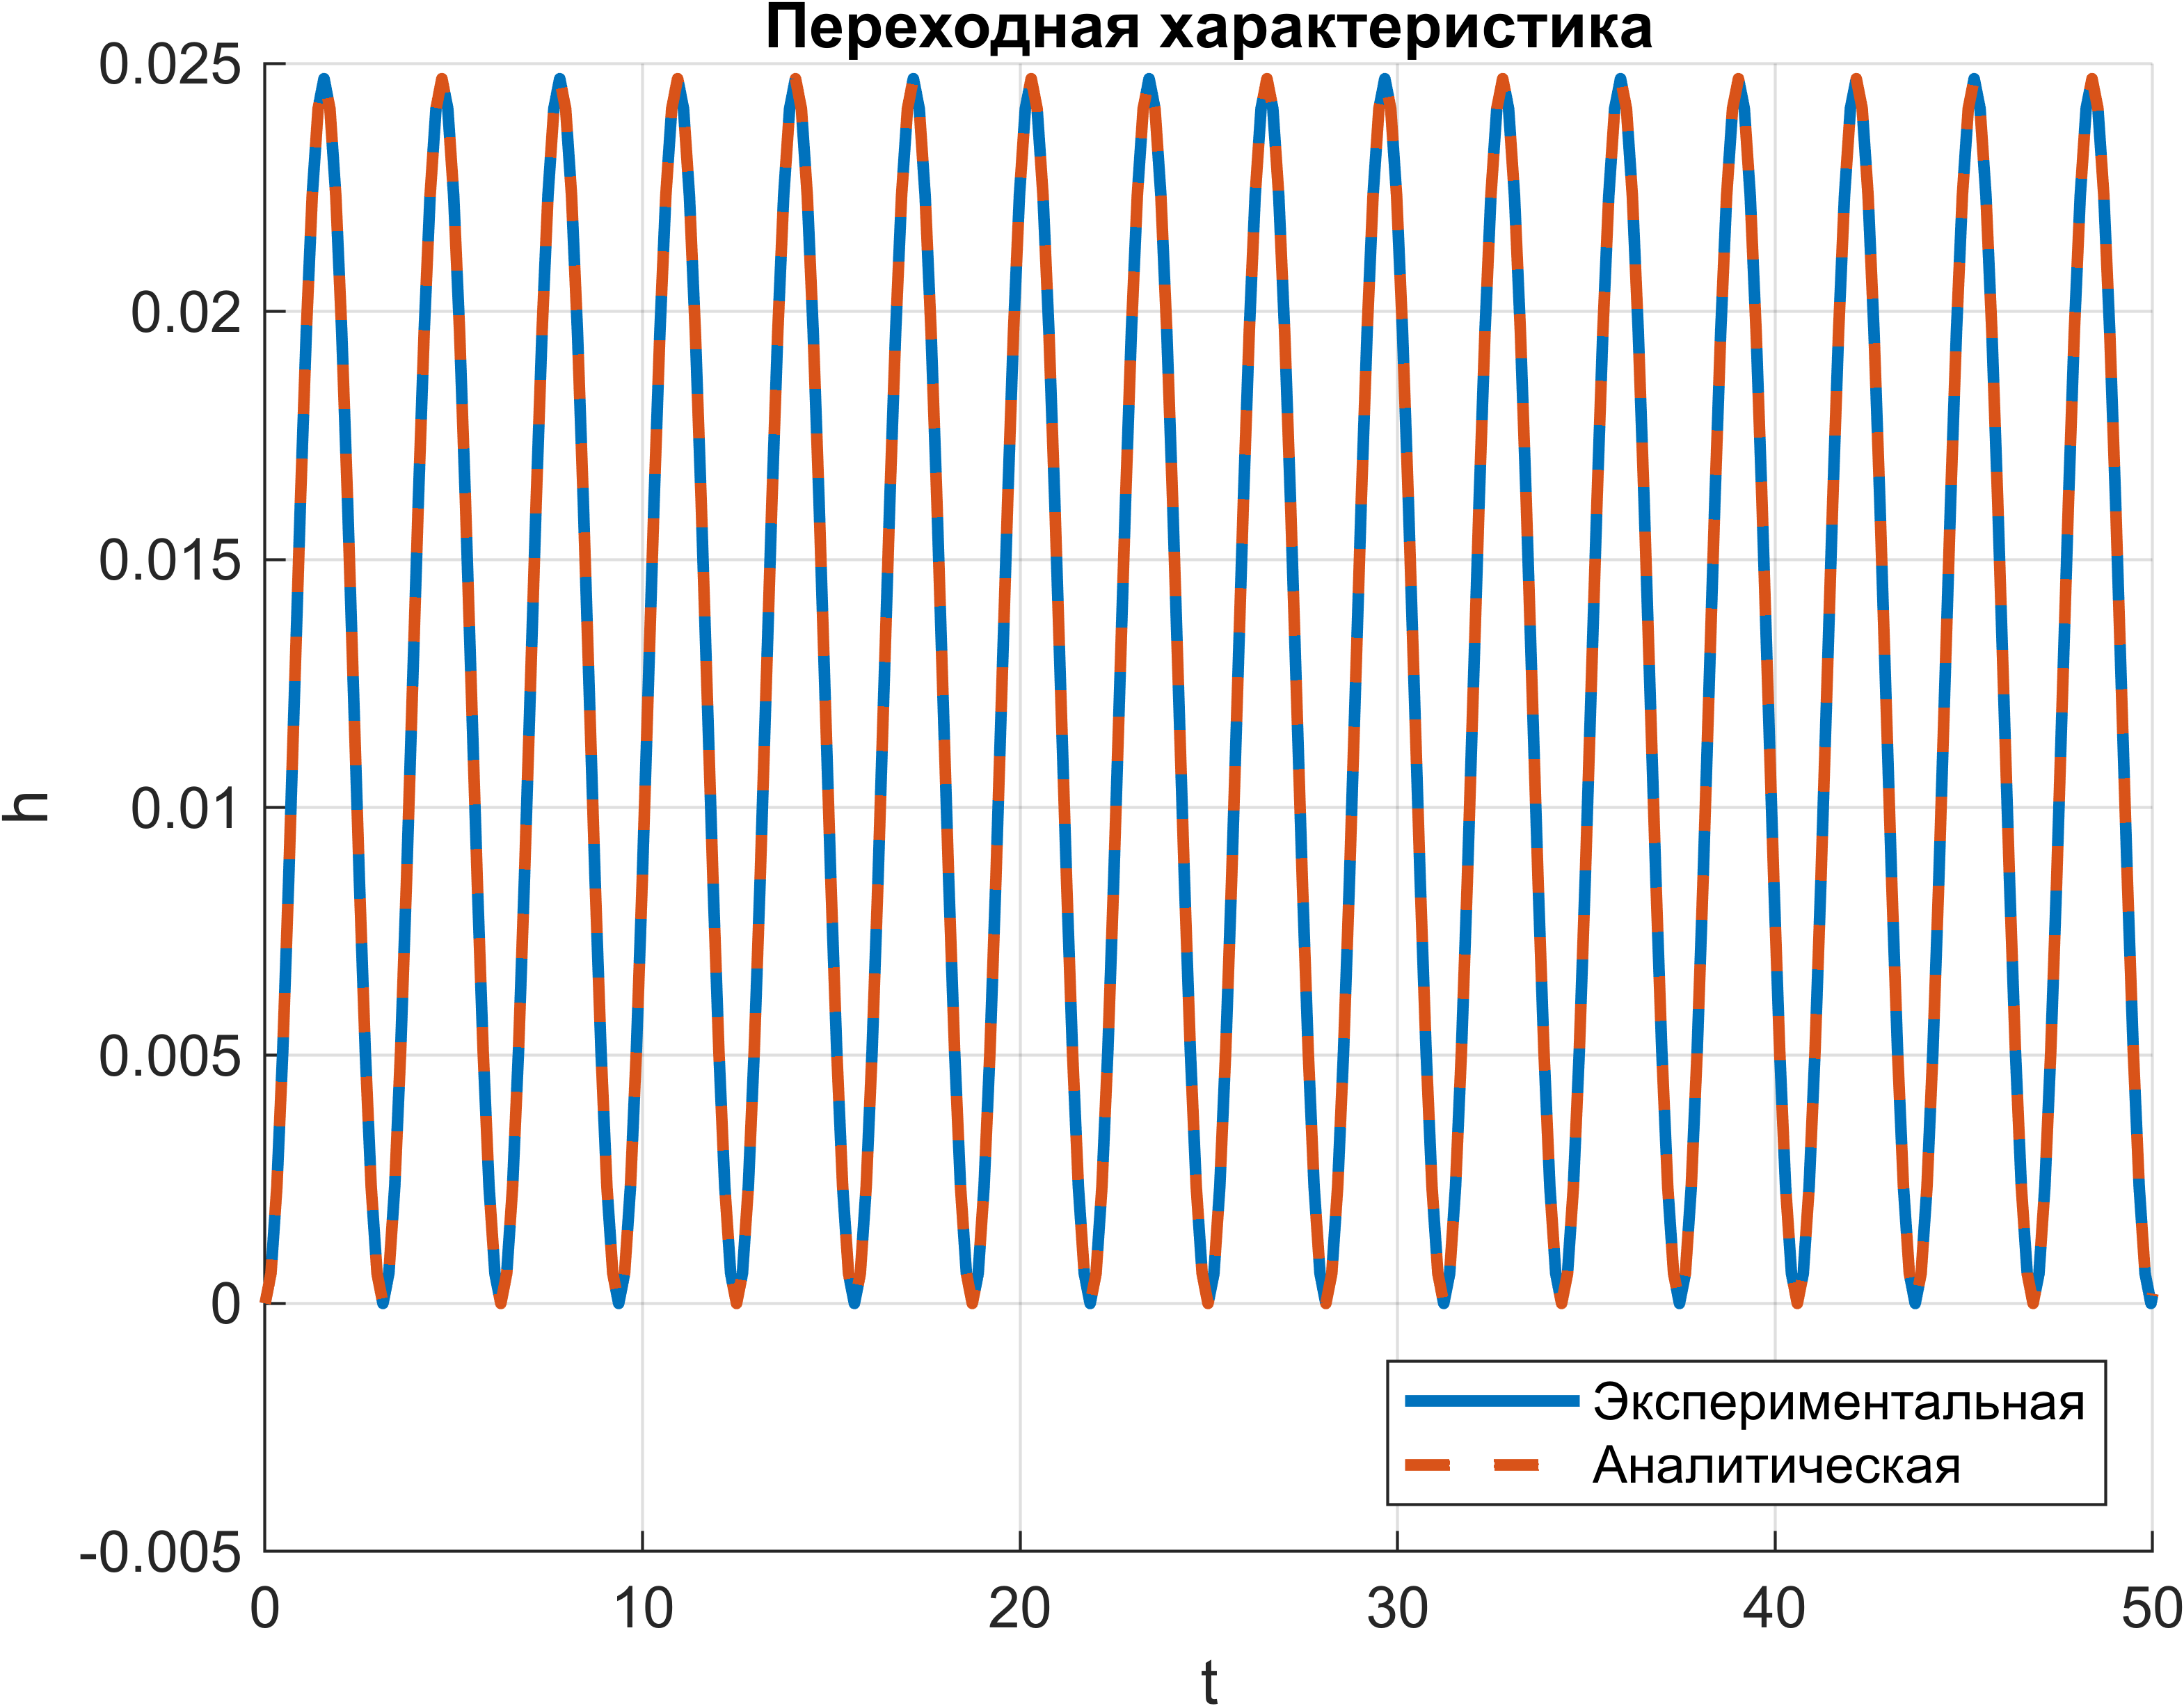
\includegraphics[width=0.75\textwidth, trim={0cm 0cm 0cm 0cm}]{../images/4_1.png}
    \caption{Переходная характеристика пружинного маятника}
\end{figure}

\begin{figure}[H]
    \centering
    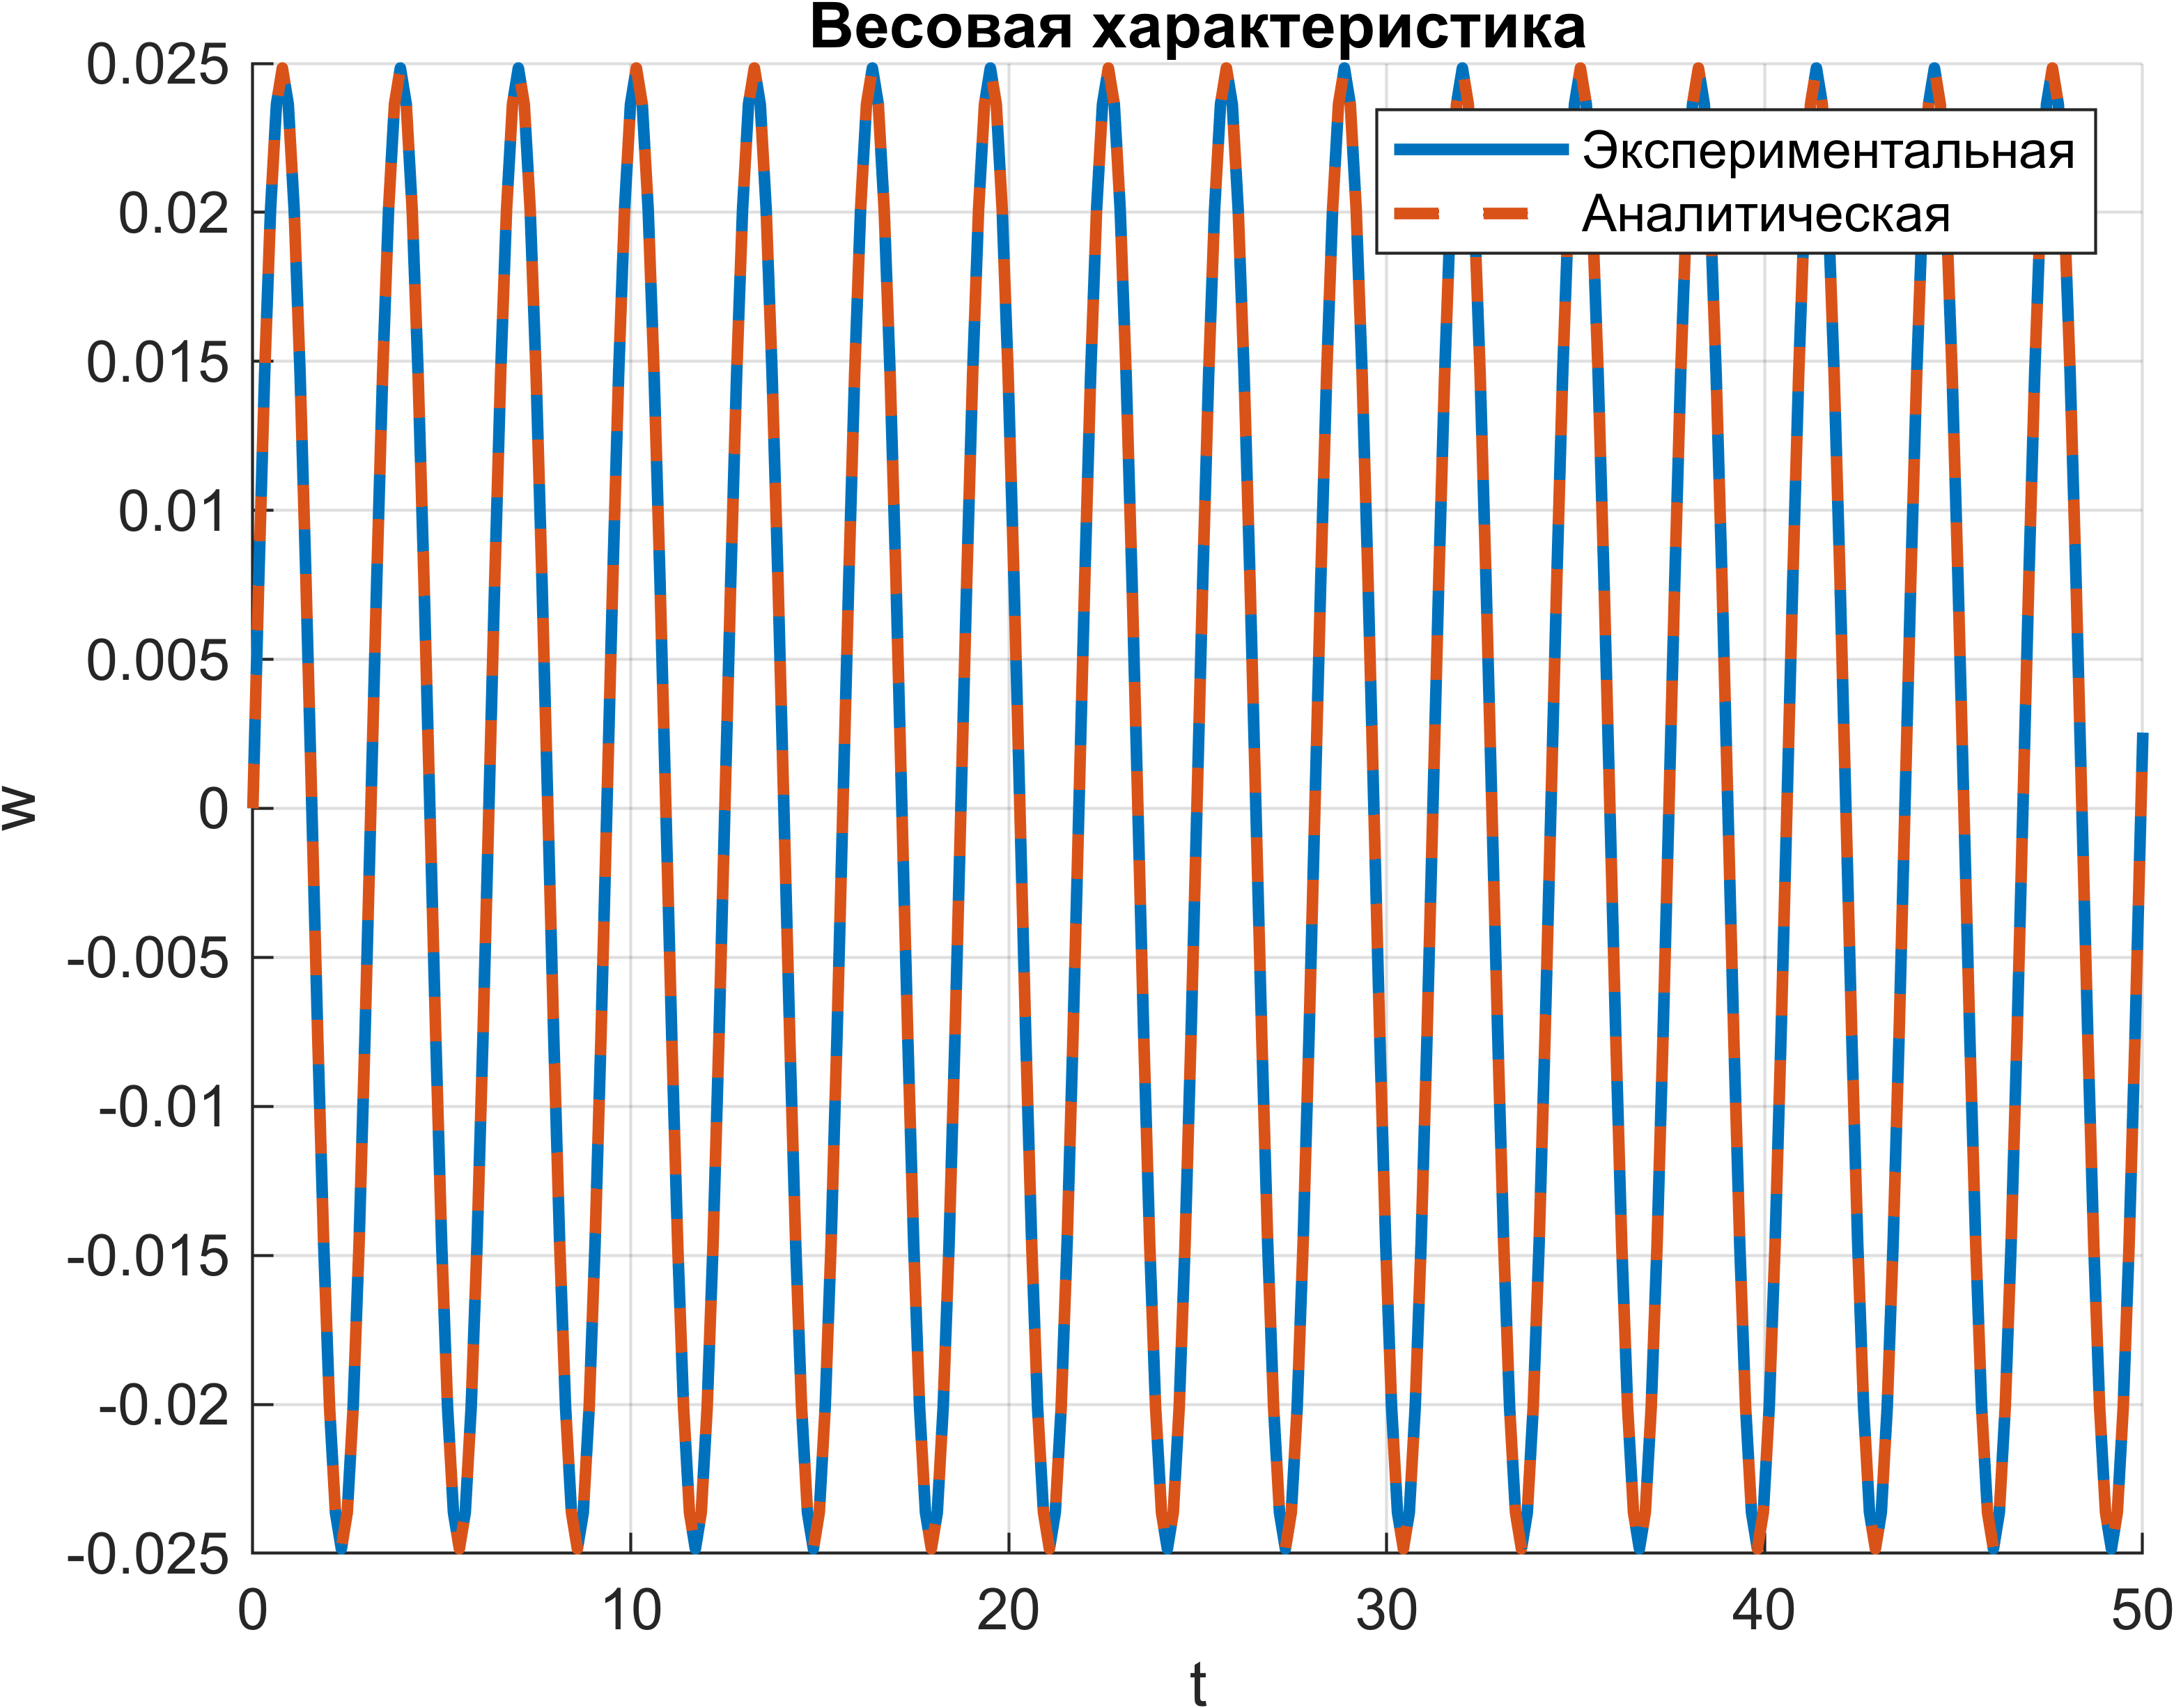
\includegraphics[width=0.75\textwidth, trim={0cm 0cm 0cm 0cm}]{../images/4_2.png}
    \caption{Весовая характеристика пружинного маятника}
\end{figure}

\section{Частотные характеристики}

Амплитудно-частотная характеристика для консервативного звена имеет вид:
\[
    A(\omega) = \frac{K}{1 - \omega^2 T^2}
\]

Логарифмическая амплитудно-частотная характеристика:
\[
    L(\omega) = 20 \lg(K) - 40 \lg(1 - \omega^2 T^2)
\]

Фазо-частотная характеристика для консервативного звена имеет вид:
\[
\varphi(\omega) = -a\pi 
\begin{cases} 
a = 0, & \omega < T^{-1} \\ 
a = 1, & \omega > T^{-1} 
\end{cases}
\]

\begin{figure}[H]
    \centering
    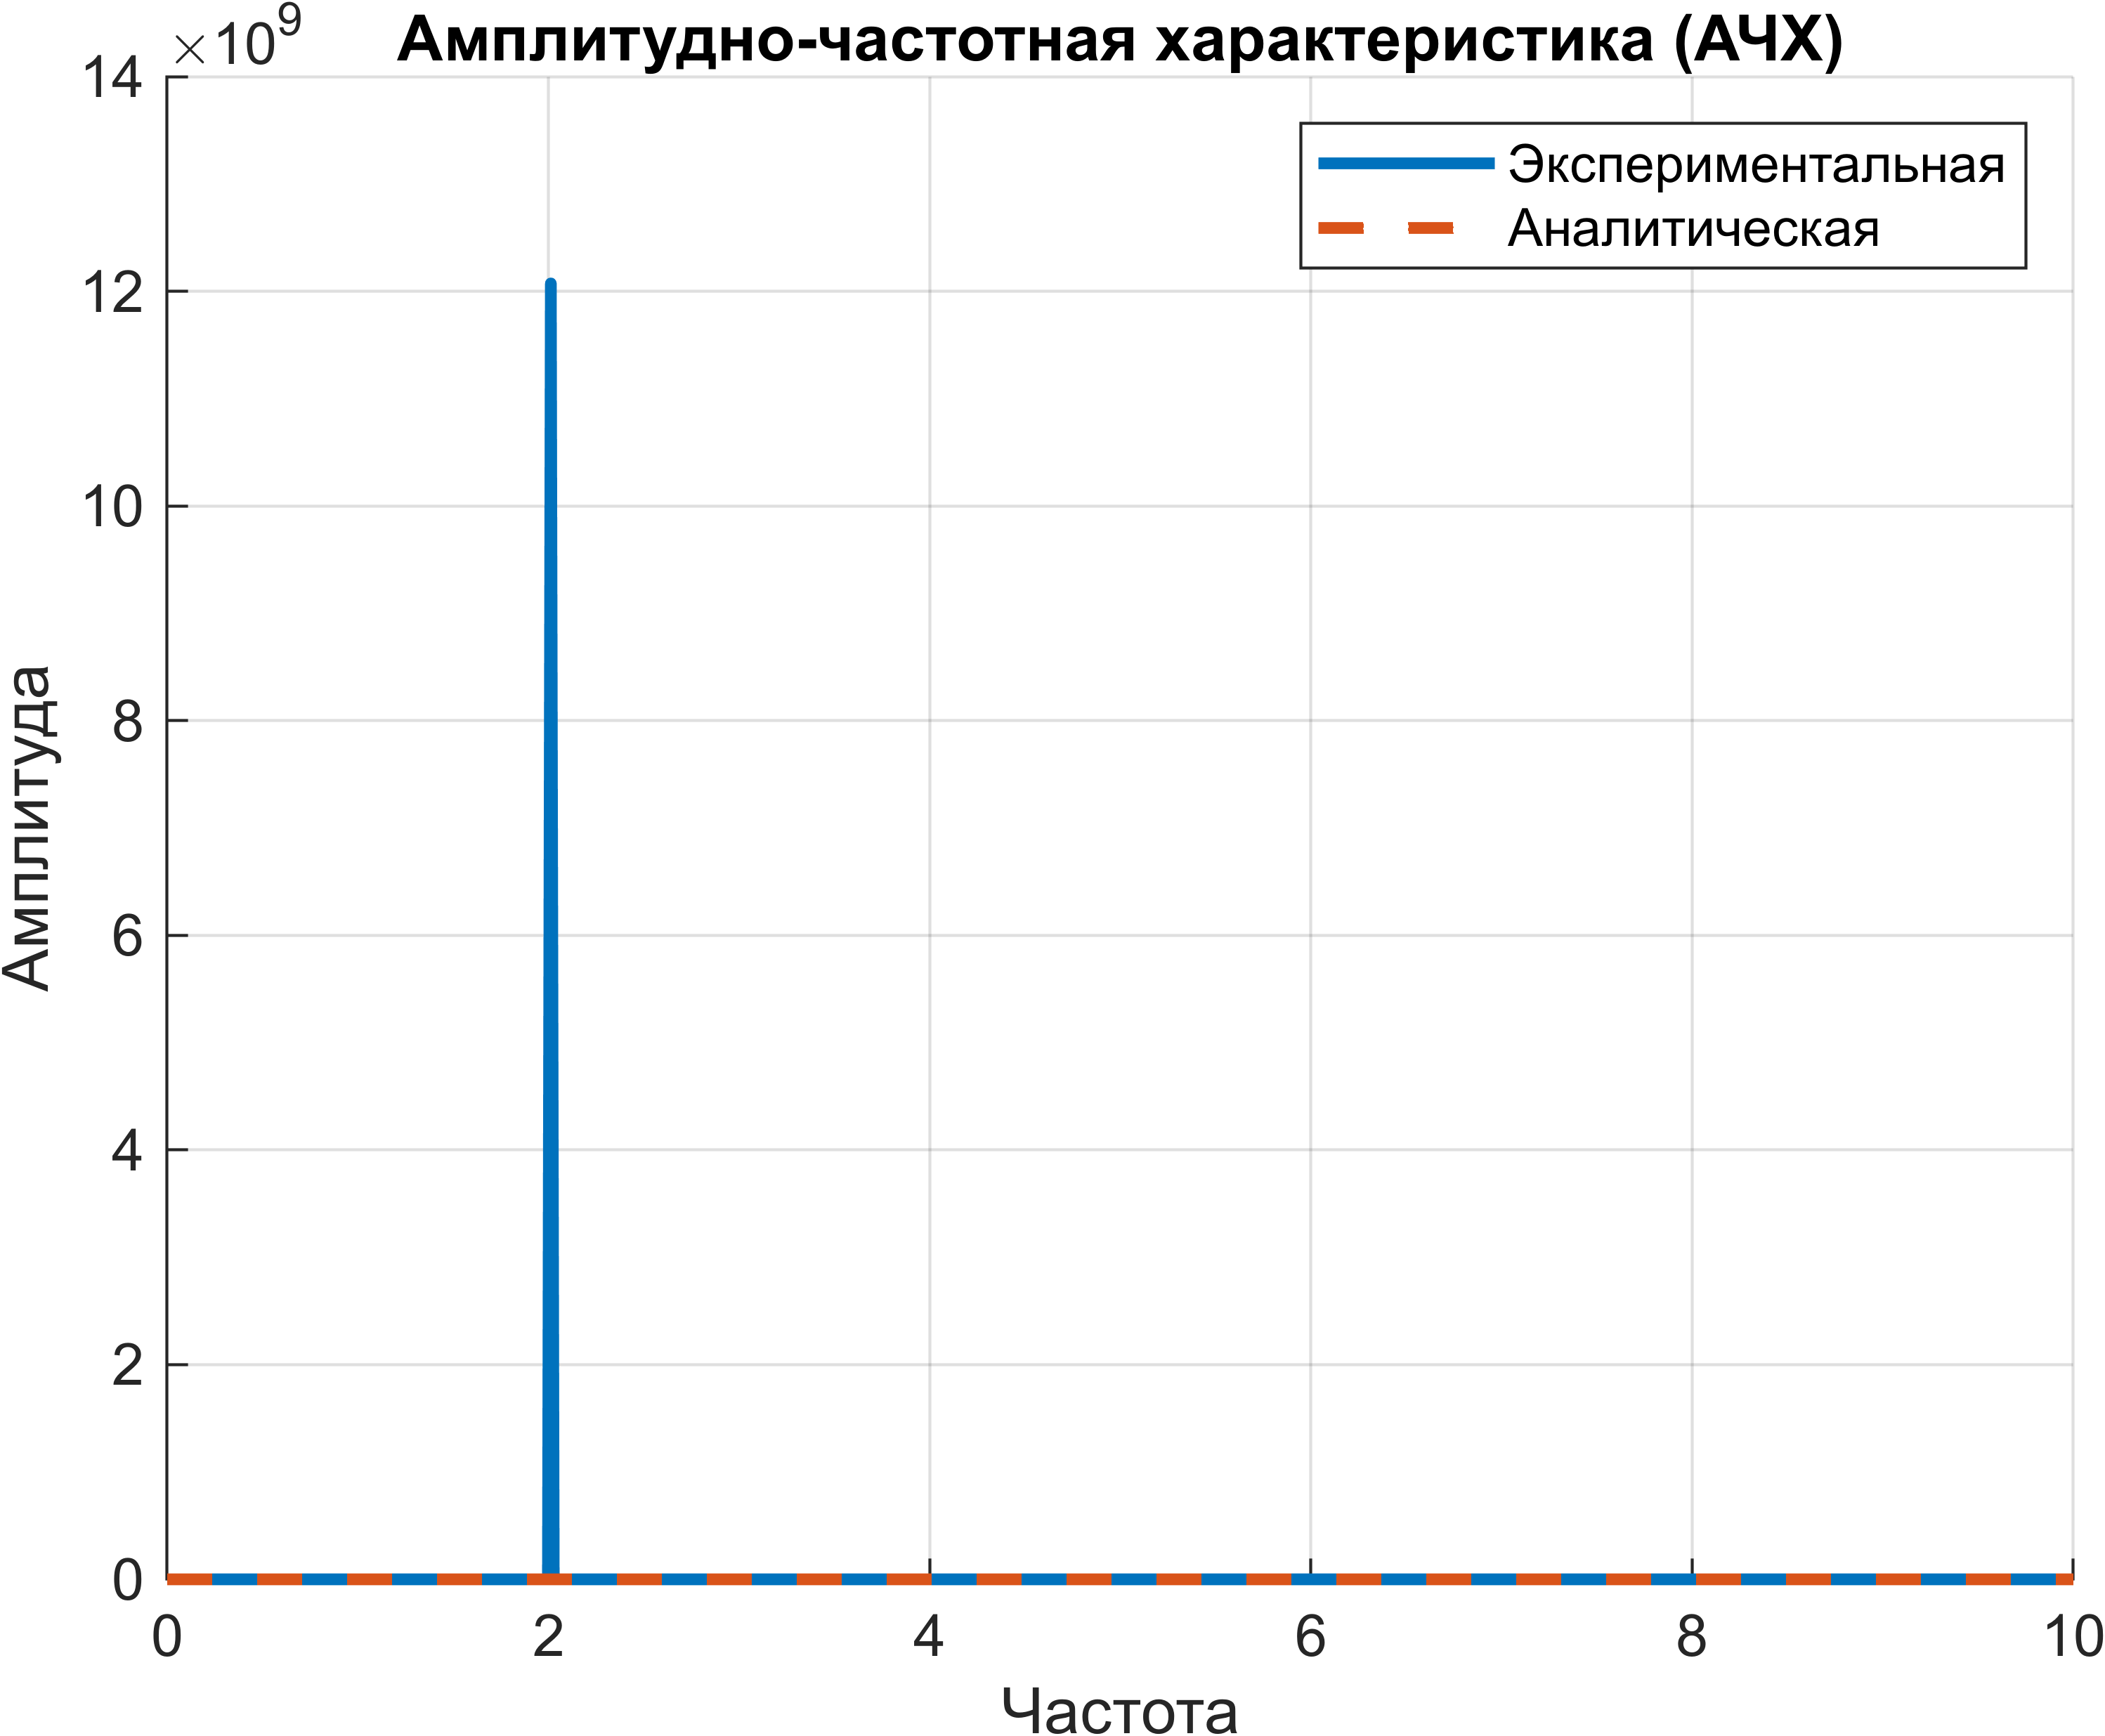
\includegraphics[width=0.75\textwidth, trim={0cm 0cm 0cm 0cm}]{../images/4_3.png}
    \caption{Амплитудно-частотная характеристика пружинного маятника}
\end{figure}

\begin{figure}[H]
    \centering
    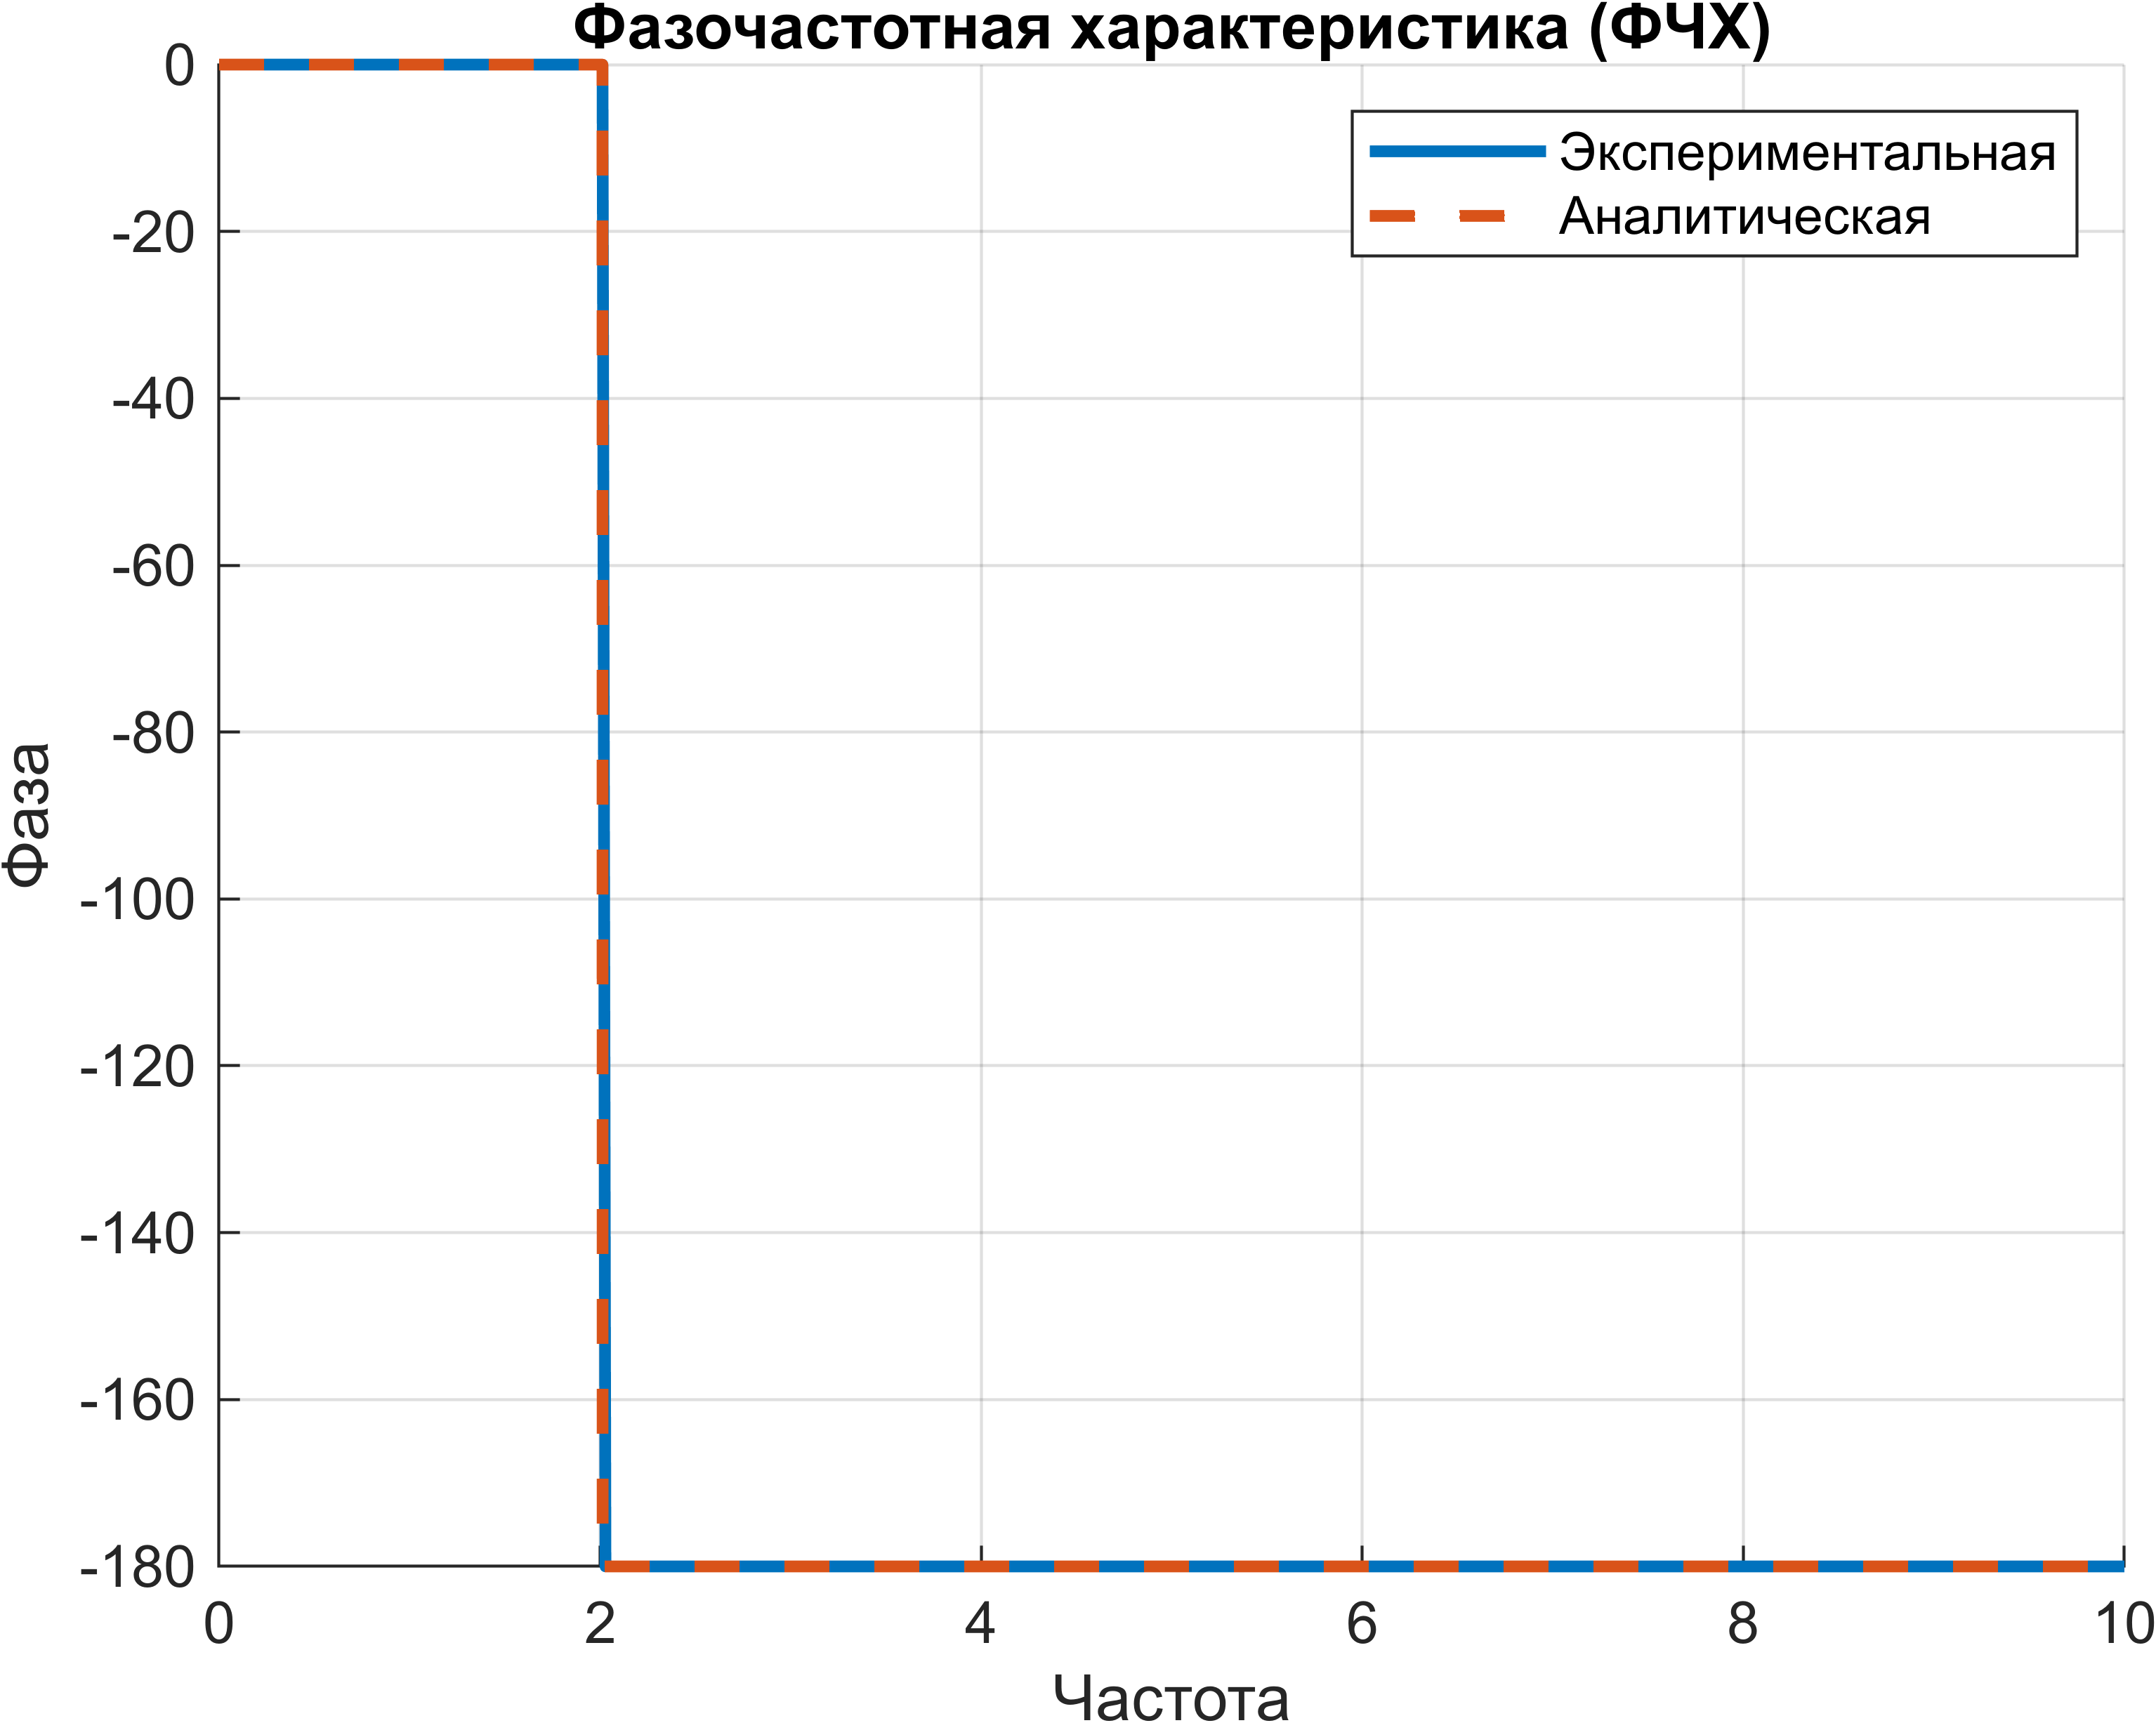
\includegraphics[width=0.75\textwidth, trim={0cm 0cm 0cm 0cm}]{../images/4_4.png}
    \caption{Фазо-частотная характеристика пружинного маятника}
\end{figure}

\begin{figure}[H]
    \centering
    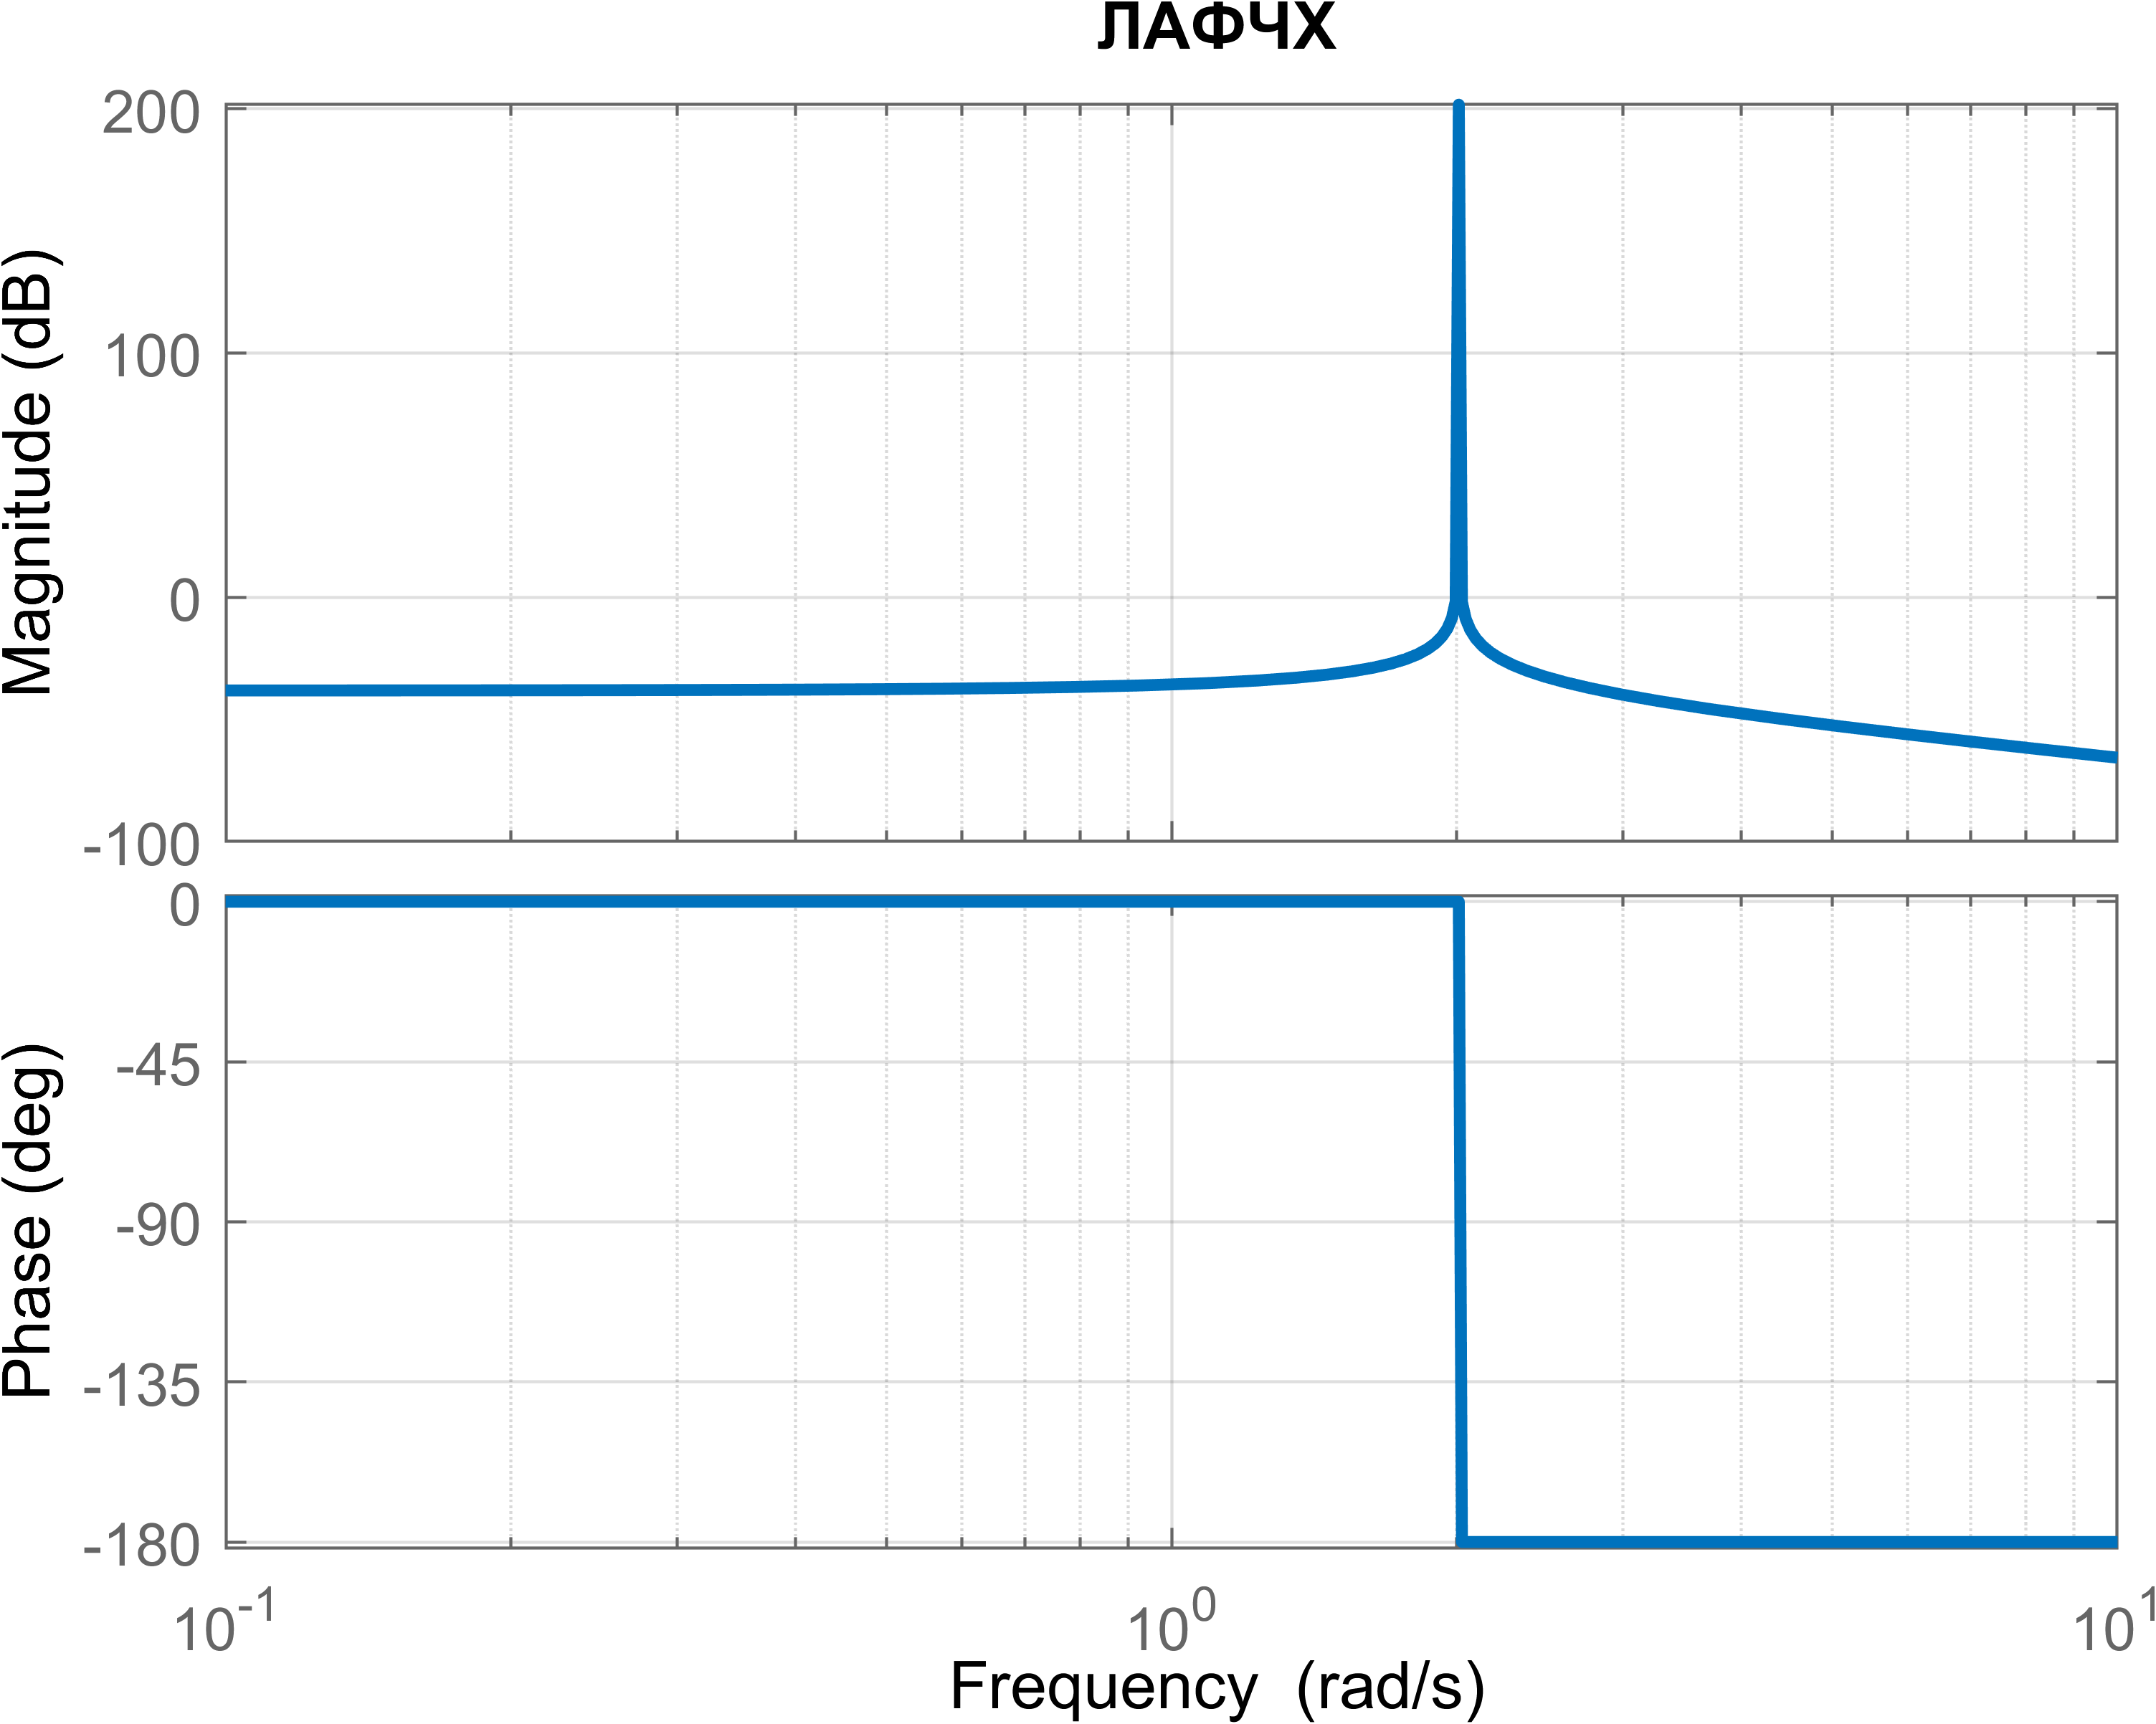
\includegraphics[width=0.75\textwidth, trim={0cm 0cm 0cm 0cm}]{../images/4_5.png}
    \caption{Логарифмическая амплитудно-фазо-частотная характеристика пружинного маятника}
\end{figure}
\endinput
